\setlength{\columnsep}{3pt}
\begin{flushleft}

\begin{figure}[h!]
	\centering
	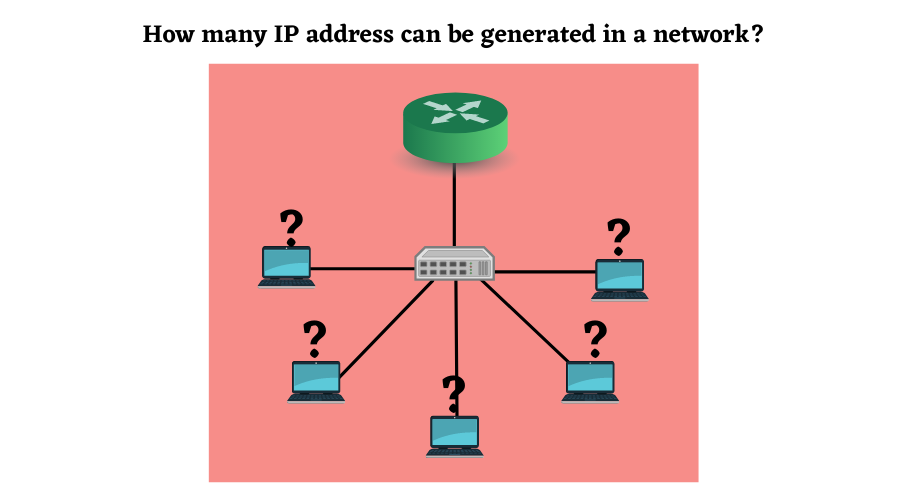
\includegraphics[scale=.7]{content/chapter14/images/how_many.png}
	\caption{Host IP}
	\label{fig:localhost}
\end{figure}	

\begin{itemize}
	\item To calculate number of host IP address in any network:
	\bigskip
	\begin{tcolorbox}[breakable,notitle,boxrule=-0pt,colback=yellow,colframe=yellow]
		\color{black}
		\fontdimen2\font=1em
		Formula: $2^n$ - 2
		\fontdimen2\font=4pt
	\end{tcolorbox}
	In this formula:
	\begin{itemize}
		\item 	\textbf{n} = \textbf{host id bits}
		\item The \textbf{-2} is to remove network address and broadcast address
	\end{itemize}
\end{itemize}


\newpage
\textbf{Examples 1}
\newline
If you have an IP address \textbf{18.6.7.8}, how will you determine total number of host IP address in it's network?	

\textbf{Solution}: From IP address \textbf{18.6.7.8}, you can conclude -
\begin{tcolorbox}[breakable,notitle,boxrule=-0pt,colback=pink,colframe=pink]	
	\color{black}
	Class: \textbf{A}
	\newline
	Netmask: \textbf{255.0.0.0}
	\newline
	Host ID bits: \textbf{24}
	\newline
	Total number of host IP address: \textbf{$2^\textbf{24}$ - 2 = 1,67,77,214}
\end{tcolorbox}

\begin{figure}[h!]
	\centering
	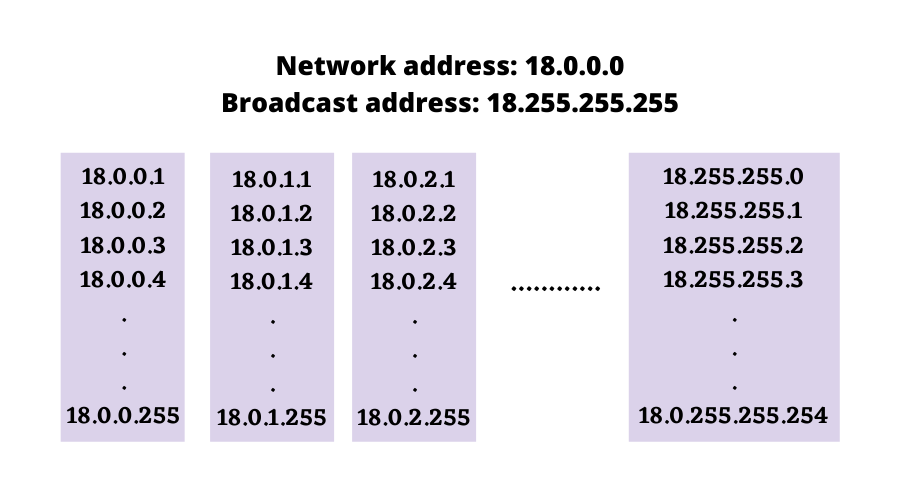
\includegraphics[scale=.7]{content/chapter14/images/calculation.png}
	\caption{Total IP address for 18.0.0.0 network}
	\label{fig:network1}
\end{figure}	

\newpage

\textbf{Examples 2}

If you have an IP address \textbf{160.7.27.10}, how will you determine total number of host IP address in it's network?	

\textbf{Solution}: From IP address \textbf{160.7.27.10}, you can conclude:
\begin{tcolorbox}[breakable,notitle,boxrule=-0pt,colback=pink,colframe=pink]
	\color{black}
	Class: \textbf{B}
	\newline
	Netmask: \textbf{255.255.0.0}
	\newline
	Host ID bits: \textbf{16}
	\newline
	Total number of host IP address: \textbf{$2^\textbf{16}$} \textbf{- 2 = 65534}
\end{tcolorbox}	

\begin{figure}[h!]
	\centering
	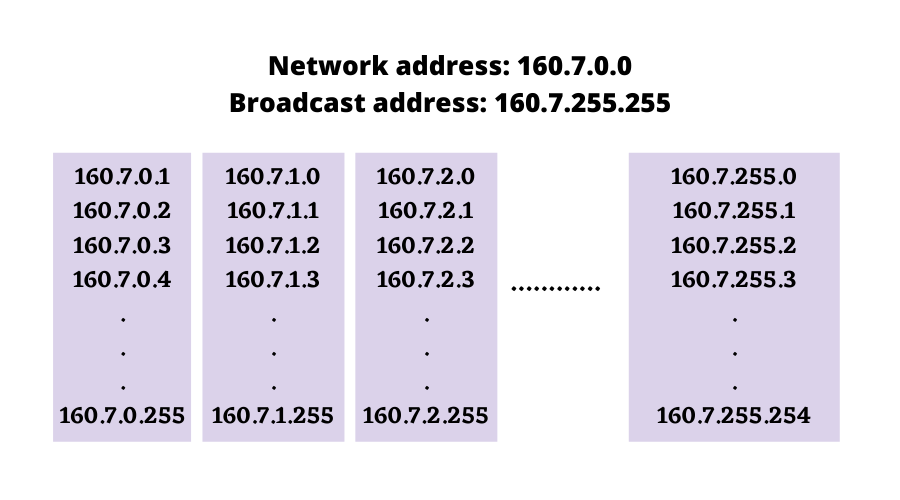
\includegraphics[scale=.7]{content/chapter14/images/calculation2.png}
	\caption{Total IP address for 160.7.0.0 network}
	\label{fig:network1}
\end{figure}	

\newpage
\textbf{Examples 3}

If you have an IP address \textbf{223.17.28.0}, how will you determine total number of host IP address in it's network?	

\textbf{Solution}: From IP address \textbf{223.17.28.0}, you can conclude:
\begin{tcolorbox}[breakable,notitle,boxrule=-0pt,colback=pink,colframe=pink]
	\color{black}
	Class: \textbf{C}
	\newline
	Netmask: \textbf{255.255.255.0}
	\newline
	Host ID bits: \textbf{8}
	\newline
	Total number of host IP address: \textbf{$2^\textbf{8}$} \textbf{- 2 = 254}
\end{tcolorbox}	

\begin{figure}[h!]
	\centering
	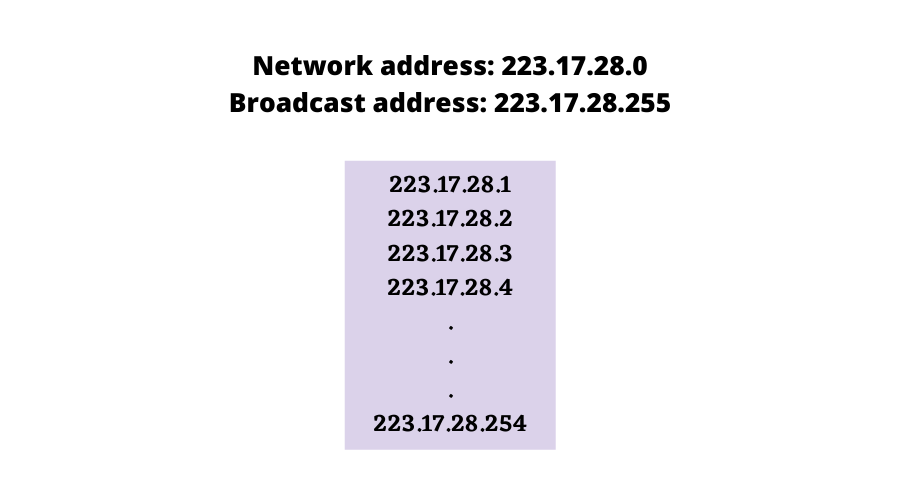
\includegraphics[scale=.7]{content/chapter14/images/calculation3.png}
	\caption{Total IP address for 223.17.28.0 network}
	\label{fig:network1}
\end{figure}	

\end{flushleft}
\newpage
